\documentclass[tikz,margin=2pt]{standalone}
\usepackage{xcolor}
\usepackage{helvet}
\usepackage{pgfplots,pgfplotstable}
%\pgfplotsset{compat=newest}
\pgfplotsset{compat=1.18}

\pgfplotsset{
  xticklabel={$\mathsf{\pgfmathprintnumber{\tick}}$},
  yticklabel={$\mathsf{\pgfmathprintnumber{\tick}}$},
}
\pgfplotsset{ 
    every non boxed x axis/.append style={x axis line style=-},
    every non boxed y axis/.append style={y axis line style=-},
}

\definecolor{c1}{RGB}{0,147,132}
\definecolor{c2}{RGB}{102,102,102}

\definecolor{themeBlue}{RGB}{1, 103, 143}
\definecolor{themeOrange}{RGB}{221, 109, 16}
\definecolor{themeTeal}{RGB}{18, 54, 69}
\definecolor{themeGrey}{RGB}{120, 121, 124}

\usepackage{tikz}
\usetikzlibrary{shapes,arrows,calc,datavisualization, arrows.meta}

\renewcommand\familydefault\sfdefault

\begin{document}
  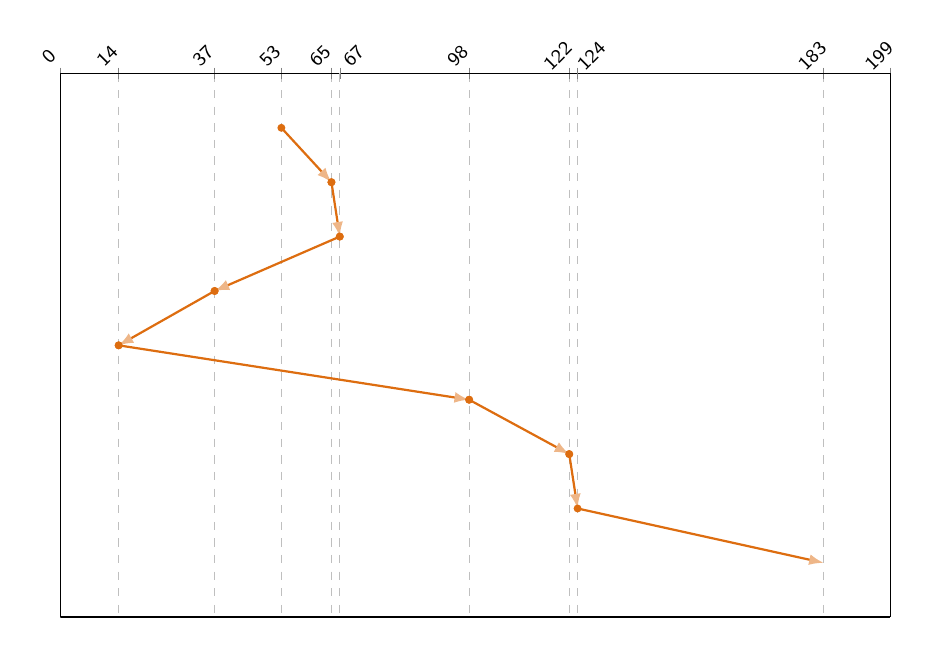
\begin{tikzpicture}[font=\sffamily]
    \begin{axis} [
    	 mark size=1.0pt,
         axis x line  = top,
         width        = 1\textwidth,
         height       = .7\textwidth,
         ymax         = 10,
         ymin         = 0,
         ytick        = \empty,
         y dir        = reverse,
         xmax         = 199,
         xmin         = 0,
         xtick        = {0,14,37,53,65,98,122,183,199},
         extra x ticks = {67, 124},
         extra x tick style={
            xticklabel style={anchor=south, yshift=-1.5ex, xshift=1.5ex}
         },
         xmajorgrids,
         grid style=dashed,
         x tick label style = {
            font=\sffamily\scriptsize,
            rotate=45,
            anchor=south
         },
         execute at begin axis = {
            \draw[thick] (rel axis cs:0,0) -- (rel axis cs:1,0);
         },
       ]

      \foreach \x [count=\y from 1, remember=\x as \lastx (initially 124)] in {122, 98, 14, 37,  67, 65, 53} {
        \pgfmathtruncatemacro{\realy}{9 - \y};
        \pgfmathtruncatemacro{\lasty}{\realy - 1};
        \addplot[color=themeOrange, thick, mark=*, arrows = {Latex[color=themeOrange!50,scale=.8]-}] coordinates {
            (\lastx, \realy)
            (\x, \lasty)
          };
      }
      \addplot[color=themeOrange, thick, arrows = {-Latex[color=themeOrange!50,scale=.8, ]}] coordinates {
        (124, 8)
        (183, 9)
      };
    \end{axis}
   
   \end{tikzpicture}
\end{document}
